\documentclass[]{article}

\usepackage[margin=0.5in]{geometry}
\usepackage{tikz}
\usetikzlibrary{arrows}

\tikzset{ shorten <>/.style={ shorten >=#1, shorten <=#1 } }

\begin{document}

\resizebox {\linewidth} {!} {
	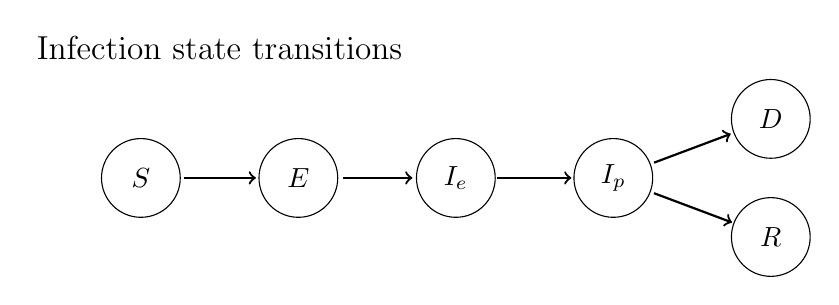
\begin{tikzpicture}
	%\draw[thick,dotted] (0,-0.25) rectangle (7.5, 1.25);
	\node at (1, 0) [label=\large Infection state transitions] {};
	\draw (0, -1.25) circle(0.5) node (S) {$ S$};
	\draw (2, -1.25) circle(0.5) node (E) {$ E $};
	\draw (4, -1.25) circle(0.5) node (Ie) {$ I_{e} $};
	\draw (6, -1.25) circle(0.5) node (Ip) {$ I_{p} $};
	\draw (8, -0.5) circle(0.5) node (D) {$ D $};
	\draw (8, -2) circle(0.5) node (R) {$ R $};

	\draw [thick,->,shorten >=2.75mm,shorten <=3mm] (S) -- (E) node[midway,above] {};
	\draw [thick,->,shorten <=3mm,shorten >=2.75mm] (E) -- (Ie) node[midway,above] {};
	\draw [thick,->,shorten <>=2.5mm] (Ie) -- (Ip) node[midway,above] {};
	\draw [thick,->,shorten >=2.5mm, shorten <= 2.5mm] (Ip) -- (R) node[midway,above] {};
	\draw [thick,->,shorten >=2.5mm, shorten <= 2.5mm] (Ip) -- (D) node[midway,above] {};
	\end{tikzpicture}
}
\end{document}
